% !TeX program = xelatex
\documentclass[11pt,a4paper]{article}

% -------------------------------------------------
% Packages
% -------------------------------------------------
\usepackage{kotex}
\usepackage{fontspec}
\usepackage{amsmath,amssymb,bm,mathtools}
\usepackage[left=24mm,right=24mm,top=23mm,bottom=25mm]{geometry}
\usepackage{booktabs,array}
\usepackage{enumitem}
\usepackage{setspace}
\usepackage{xcolor}
\usepackage{tikz}
\usetikzlibrary{positioning,arrows.meta,calc,fit}
\usepackage[most]{tcolorbox}
\usepackage{listings}
\usepackage{hyperref}
\usepackage{fancyhdr}

\setstretch{1.14}
\setlength{\parindent}{0pt}
\setlength{\parskip}{0.55em}

% -------------------------------------------------
% Colors and boxes
% -------------------------------------------------
\definecolor{deepblue}{RGB}{34,71,120}
\definecolor{softblue}{RGB}{239,246,253}
\definecolor{softgray}{RGB}{246,247,249}
\definecolor{softgreen}{RGB}{239,249,242}
\definecolor{softyellow}{RGB}{255,249,229}
\definecolor{codegray}{RGB}{248,248,248}

\newtcolorbox{keybox}[1][]{
  colback=softblue,
  colframe=deepblue,
  boxrule=0.7pt,
  arc=2mm,
  title=#1,
  fonttitle=\bfseries
}

\newtcolorbox{thinkbox}[1][]{
  colback=softyellow,
  colframe=orange!70!black,
  boxrule=0.6pt,
  arc=2mm,
  title=#1,
  fonttitle=\bfseries
}

\newtcolorbox{remarkbox}[1][]{
  colback=softgray,
  colframe=black!45,
  boxrule=0.5pt,
  arc=2mm,
  title=#1,
  fonttitle=\bfseries
}

\newtcolorbox{mlbox}[1][]{
  colback=softgreen,
  colframe=green!45!black,
  boxrule=0.6pt,
  arc=2mm,
  title=#1,
  fonttitle=\bfseries
}

% -------------------------------------------------
% Code style
% -------------------------------------------------
\lstdefinestyle{pythonstyle}{
  language=Python,
  backgroundcolor=\color{codegray},
  basicstyle=\ttfamily\small,
  keywordstyle=\bfseries,
  commentstyle=\itshape\color{black!60},
  stringstyle=\color{black!75},
  numbers=left,
  numberstyle=\tiny\color{black!55},
  numbersep=8pt,
  frame=single,
  rulecolor=\color{black!25},
  breaklines=true,
  showstringspaces=false,
  tabsize=4,
  columns=fullflexible,
  keepspaces=true
}
\lstset{style=pythonstyle}

% -------------------------------------------------
% Math commands
% -------------------------------------------------
\newcommand{\R}{\mathbb{R}}
\newcommand{\grad}{\nabla}
\newcommand{\vect}[1]{\bm{#1}}
\newcommand{\T}{^{\mathsf T}}
\newcommand{\dd}{\,\mathrm d}
\newcommand{\loss}{\mathcal{L}}

% -------------------------------------------------
% Header / footer
% -------------------------------------------------
\pagestyle{fancy}
\fancyhf{}
\lhead{Introduction to Deep Learning and Practice}
\rhead{Chain Rule and Backpropagation}
\cfoot{\thepage}
\renewcommand{\headrulewidth}{0.4pt}
\setlength{\headheight}{14pt}

\hypersetup{
  colorlinks=true,
  linkcolor=deepblue,
  urlcolor=deepblue
}

% -------------------------------------------------
% Document
% -------------------------------------------------
\begin{document}

\begin{center}
{\LARGE\bfseries 합성함수 미분법에서 Backpropagation까지}\\[0.35em]
{\Large Chain Rule $\rightarrow$ Gradient/Jacobian $\rightarrow$ Backpropagation in Linear Regression}\\[0.8em]
\end{center}

\vspace{0.4em}

\begin{keybox}[이번 주의 핵심 질문]
딥러닝에서 학습한다는 것은 결국 손실함수 $L$을 모델 파라미터에 대해 미분하고,
그 미분값을 이용하여 파라미터를 수정하는 과정이다. 그렇다면 수많은 함수가 반복적으로
합성된 신경망에서
\[
\frac{\partial L}{\partial \theta}
\]
를 어떻게 체계적으로 계산할 수 있을까?

이번 주에는 그 출발점이 되는 \textbf{chain rule}을 일변수에서 다변수로 확장하고,
가장 단순한 학습모델인 선형회귀를 계산 그래프로 다시 해석하여
\textbf{forward propagation과 backward propagation의 원형}을 직접 유도하고 구현한다.
\end{keybox}

\subsection*{학습목표}
이 주차가 끝나면 다음을 설명하고 직접 계산할 수 있어야 한다.
\begin{enumerate}[label=\arabic*.]
\item 합성함수와 chain rule을 ``변화율의 전달''이라는 관점에서 설명한다.
\item 편미분, gradient, Jacobian의 의미를 구분한다.
\item 다변수 chain rule을 scalar form과 matrix form으로 표현한다.
\item 계산 그래프(computational graph)에서 forward와 backward의 의미를 설명한다.
\item 선형회귀의 MSE loss에 대해 $\partial L/\partial w$, $\partial L/\partial b$를 chain rule로 유도한다.
\item 위 유도식을 NumPy로 직접 coding하여 gradient descent를 수행한다.

\end{enumerate}



% =================================================
\section{합성함수와 일변수 Chain Rule}
% =================================================

\subsection{합성함수와 chain rule}

변수 $x,y,z$가 다음과 같이 연결되어 있다고 하자.
\[
y=g(x), \qquad z=f(y).
\]
그러면 $z$는 결국 $x$의 함수이고,
\[
z=f(g(x))=(f\circ g)(x)
\]
로 쓸 수 있다.

\begin{center}
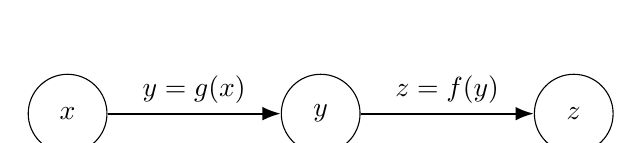
\begin{tikzpicture}[>=Latex,node distance=2.2cm]
\node[draw,circle,minimum size=10mm] (x) {$x$};
\node[draw,circle,minimum size=10mm,right=of x] (y) {$y$};
\node[draw,circle,minimum size=10mm,right=of y] (z) {$z$};
\draw[->,thick] (x) -- node[above] {$y=g(x)$} (y);
\draw[->,thick] (y) -- node[above] {$z=f(y)$} (z);
\end{tikzpicture}
\end{center}

여기에서 $y$는 단순한 기호가 아니라, $x$의 변화가 $z$로 전달되는 과정에 존재하는
\textbf{중간 변수(intermediate variable)}이다. 이 관점이 뒤에서 computational graph를 이해할 때 중요하다.


$g$가 $x$에서 미분가능하고 $f$가 $g(x)$에서 미분가능하면
\[
h(x)=f(g(x))
\]
의 도함수는
\[
\boxed{
 h'(x)=f'(g(x))g'(x)
}
\]
이다.

중간 변수 $y=g(x)$를 사용하면
\[
\boxed{
\frac{dz}{dx}
=
\frac{dz}{dy}\frac{dy}{dx}
}
\]
로 쓸 수 있다.

연쇄법칙은 영어로 \textbf{chain rule}이라 하는데 이는 다음과 같이
이해할 수 있다.

\begin{figure}[ht]
    \centering
    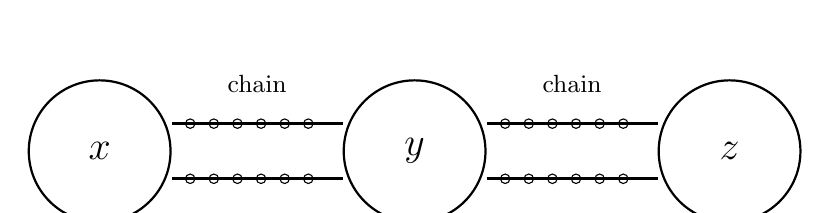
\begin{tikzpicture}[scale=1.0]

        % gears
        \node[
            circle,
            draw,
            minimum size=1.8cm,
            line width=0.8pt
        ] (x) at (0,0) {\Large $x$};

        \node[
            circle,
            draw,
            minimum size=1.8cm,
            line width=0.8pt
        ] (y) at (4,0) {\Large $y$};

        \node[
            circle,
            draw,
            minimum size=1.8cm,
            line width=0.8pt
        ] (z) at (8,0) {\Large $z$};

        % chain x-y : upper and lower strands
        \draw[line width=1.1pt]
            ($(x.east)+(0,0.35)$)
            --
            ($(y.west)+(0,0.35)$);

        \draw[line width=1.1pt]
            ($(x.east)+(0,-0.35)$)
            --
            ($(y.west)+(0,-0.35)$);

        % chain y-z
        \draw[line width=1.1pt]
            ($(y.east)+(0,0.35)$)
            --
            ($(z.west)+(0,0.35)$);

        \draw[line width=1.1pt]
            ($(y.east)+(0,-0.35)$)
            --
            ($(z.west)+(0,-0.35)$);

        % small chain links: x-y
        \foreach \s in {1.15,1.45,...,2.85}{
            \draw (\s,0.35) circle (0.06);
            \draw (\s,-0.35) circle (0.06);
        }

        % small chain links: y-z
        \foreach \s in {5.15,5.45,...,6.85}{
            \draw (\s,0.35) circle (0.06);
            \draw (\s,-0.35) circle (0.06);
        }

        % labels
        \node at (2,0.85) {\small chain};
        \node at (6,0.85) {\small chain};

    \end{tikzpicture}
\end{figure}

크기가 다른 세 개의 톱니바퀴 $x$, $y$, $z$가 있다고 하자.
$x$는 $y$에 체인으로 연결되어 있고,
$y$는 $z$에 체인으로 연결되어 있다고 하자.
$x$를 돌리면 $y$가 돌아가고 $y$에 연결된 $z$가 돌아가게 되므로,
중간 과정 $y$를 생략하고 생각하면 톱니바퀴 $z$의 변화는
$x$에 의해 결정된다.

만약 $x$, $y$, $z$의 톱니바퀴 수가,
$x$가 한 바퀴 돌아가면 $y$가 두 바퀴 돌아가고,
$y$가 한 바퀴 돌아갈 때 $z$는 세 바퀴 돌아가는 비율로
정해져 있다면, $x$가 두 바퀴 돌면 $z$는 몇 바퀴 돌아가겠는가?

이를 수학적으로 생각하면 다음과 같다.

\[
\begin{aligned}
x\text{ 변화}:y\text{ 변화}=1:2
&\qquad\Longleftrightarrow\qquad
\frac{dy}{dx}=2,
\\[0.5em]
y\text{ 변화}:z\text{ 변화}=1:3
&\qquad\Longleftrightarrow\qquad
\frac{dz}{dy}=3.
\end{aligned}
\]

따라서,

\[
x\text{ 변화}:z\text{ 변화}=1:6
\]

이고,

\[
\frac{dz}{dx}
=
\frac{dz}{dy}\frac{dy}{dx}
=
3\times 2
=
6.
\]

그러므로,

\[
\begin{aligned}
\Delta z
&=
\left(
z\text{의 }y\text{에 대한 변화율}
\right)
\times
\Delta y
\\[0.4em]
&=
\frac{dz}{dy}\Delta y
\\[0.4em]
&=
\frac{dz}{dy}
\left(
y\text{의 }x\text{에 대한 변화율}
\right)
\Delta x
\\[0.4em]
&=
\frac{dz}{dy}
\frac{dy}{dx}
\Delta x .
\end{aligned}
\]

로 생각할 수 있고, 따라서 $x$가 두 바퀴 돌면
$z$는 $12$바퀴가 돌아갈 것이다.

한편 $z$를 $x$의 함수로 직접 생각하면

\[
\Delta z
\approx
\frac{dz}{dx}\Delta x
\]

이므로, 위의 식과 비교하여

\[
\boxed{
\frac{dz}{dx}
=
\frac{dz}{dy}
\frac{dy}{dx}
}
\]

인 것을 알 수 있다.

이것이 합성함수의 미분법, 즉 미분계수(변화율)

\[
\frac{dz}{dx}
=
\frac{dz}{dy}
\frac{dy}{dx}
\]

의 의미이다. 이 비유의 핵심은 중간 변수 $y$를 거치면서 \textbf{변화율이 연쇄적으로 전달된다}는 데 있다.

또한 derivative는 단순한 기호 조작이 아니라
\[
\boxed{\text{입력의 작은 변화($\Delta x$)가 출력의 변화($\Delta z$)로 얼마나 증폭 또는 축소되는가}}
\]
를 나타내는 \textbf{sensitivity}이다. 

\subsection{Local linearization으로 보는 미분}

미분가능한 함수 $f$는 $x$ 근처에서
\[
f(x+\Delta x)
=
f(x)+f'(x)\Delta x+o(|\Delta x|)
\]
로 근사된다. 즉,
\[
\boxed{\Delta f\approx f'(x)\Delta x}
\]
이다.

두 함수 $y=g(x)$, $z=f(y)$를 각각 선형근사하면
\[
\Delta y\approx g'(x)\Delta x,
\qquad
\Delta z\approx f'(y)\Delta y,
\]
따라서
\[
\Delta z\approx f'(g(x))g'(x)\Delta x.
\]
이것이 chain rule의 가장 중요한 구조이다.

\subsection{예제}

\paragraph{예제 1.}
\[
y=(x^3+1)^2.
\]
$u=x^3+1$이라 두면 $y=u^2$이므로
\[
\frac{dy}{dx}
=
\frac{dy}{du}\frac{du}{dx}
=
2u\cdot 3x^2
=
6x^2(x^3+1).
\]

\paragraph{예제 2.}
\[
y=\sin(2x+1).
\]
$u=2x+1$이라 두면
\[
\frac{dy}{dx}
=
\cos u\cdot 2
=
2\cos(2x+1).
\]

\paragraph{예제 3. 세 단계 합성}
\[
y=\exp\!\left(\sin(x^2)\right).
\]
중간 변수를
\[
u_1=x^2,\qquad u_2=\sin u_1,\qquad y=e^{u_2}
\]
로 두면
\[
\frac{dy}{dx}
=
\frac{dy}{du_2}
\frac{du_2}{du_1}
\frac{du_1}{dx}
=
e^{u_2}\cos u_1\,(2x).
\]
따라서
\[
\boxed{
\frac{dy}{dx}
=2x\cos(x^2)e^{\sin(x^2)}
}.
\]


% ============================================================
\section{다변수함수의 연쇄법칙}
% ============================================================

% ------------------------------------------------------------
\subsection{하나의 입력변수에서 여러 중간변수를 거치는 경우}
% ------------------------------------------------------------

다변수함수
\[
z=f(x_1,x_2,\ldots,x_n)
\]
가 각 변수 $x_i$에 대하여 편미분 가능하다고 하자.

그런데 (알고보니) 각 변수 $x_i$가 다시 하나의 변수 $t$에 의하여 정해지는 함수
\[
x_i=x_i(t),
\qquad i=1,\ldots,n
\]
라고 하자. ($x_i$를 변수를 나타내는 기호와 함수 $x_i(\cdot)$를 나타내는 기호로 동시에 사용했다.)

그러면 결국 $z$는
\[
z
=
f\bigl(
x_1(t),x_2(t),\ldots,x_n(t)
\bigr)
\]
와 같이 $t$에 대한 함수가 된다. 이 관계를 graph로 나타내면 다음과 같다.

\begin{figure}[ht]
\centering
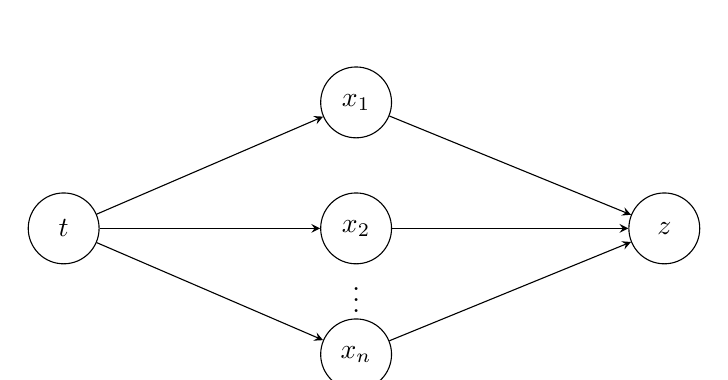
\begin{tikzpicture}[
    node distance=1.35cm and 2.5cm,
    every node/.style={
        circle,
        draw,
        minimum size=0.9cm,
        inner sep=1pt
    },
    >=stealth
]

\node (t) {$t$};

\node[right=2.8cm of t, yshift=1.6cm] (x1) {$x_1$};
\node[right=2.8cm of t] (x2) {$x_2$};
\node[right=2.8cm of t, yshift=-1.6cm] (xn) {$x_n$};

\node[right=3.0cm of x2] (z) {$z$};

\draw[->] (t) -- (x1);
\draw[->] (t) -- (x2);
\draw[->] (t) -- (xn);

\draw[->] (x1) -- (z);
\draw[->] (x2) -- (z);
\draw[->] (xn) -- (z);

\node[draw=none] at ($(x2)!0.5!(xn)$) {$\vdots$};

\end{tikzpicture}
\caption{$t$의 변화가 여러 중간변수 $x_i$를 통하여 $z$에 전달되는 구조}
\end{figure}

이 graph를 따라 생각하면,
$t$가 변할 때 $x_1,x_2,\ldots,x_n$이 각각 변하고,
각 $x_i$의 변화가 다시 $z$의 변화에 영향을 준다.

우리는 $z$의 변화는 $x_i$의 변화에 의한 영향의 총합으로 결정된다는 것을 알고 있으므로, $z$의 작은 변화 $\Delta z$는 일차근사식
\[
\Delta z
\approx
\frac{\partial z}{\partial x_1}\Delta x_1
+
\frac{\partial z}{\partial x_2}\Delta x_2
+\cdots+
\frac{\partial z}{\partial x_n}\Delta x_n
\]

으로 표현된다. 이것을 미적분학에서는 전미분 
\[
dz
= \frac{\partial z}{\partial x_1}d x_1
+
\frac{\partial z}{\partial x_2}d x_2
+\cdots+
\frac{\partial z}{\partial x_n}d x_n
\]
이라 한다.

그런데 각 $x_i$가 $t$의 함수이므로 $x_i$의 변화는 다시 $t$의 변화에 의하여 결정된다. 즉, $t$가 $\Delta t$만큼 변하면

\[
\Delta x_i
\approx
\frac{dx_i}{dt}\Delta t
\]

이다. 따라서

\[
\begin{aligned}
\Delta z
&\approx
\frac{\partial z}{\partial x_1}
\frac{dx_1}{dt}\Delta t
+
\frac{\partial z}{\partial x_2}
\frac{dx_2}{dt}\Delta t
+\cdots
+
\frac{\partial z}{\partial x_n}
\frac{dx_n}{dt}\Delta t
\\[0.5em]
&=
\left(
\frac{\partial z}{\partial x_1}
\frac{dx_1}{dt}
+
\cdots+
\frac{\partial z}{\partial x_n}
\frac{dx_n}{dt}
\right)\Delta t .
\end{aligned}
\]
즉, $t$의 작은 변화가 여러 node $x_i$에 전달되고,
각 node에서 다시 $z$로 전달되는 모든 변화의 합이
최종적인 $z$의 변화가 된다.

한편 직접 $z$를 $t$의 함수로 생각하면

\[
\Delta z
\approx
\frac{dz}{dt}\Delta t
\]

이므로 위의 식과 그 모양을 비교하면 다음을 얻을수 있다.

\[
\boxed{
\frac{dz}{dt}
=
\frac{\partial z}{\partial x_1}
\frac{dx_1}{dt}
+
\frac{\partial z}{\partial x_2}
\frac{dx_2}{dt}
+\cdots+
\frac{\partial z}{\partial x_n}
\frac{dx_n}{dt}
}
\]




각 항을 graph의 하나의 경로(path)로 생각하면

\[
t\longrightarrow x_i\longrightarrow z
\]

라는 경로를 따라 변화율이 곱해져

\[
\frac{\partial z}{\partial x_i}
\frac{dx_i}{dt}
\]

가 된다.

그리고 $t$에서 $z$로 가는 경로가 여러 개 있으므로
각 경로를 통해 전달되는 변화율을 모두 더한다.


% ------------------------------------------------------------
\subsection{여러 입력변수를 가지는 경우}
% ------------------------------------------------------------

이제 중간변수 $x_1,\ldots,x_n$이 하나의 변수 $t$가 아니라
여러 변수
\[
t_1,t_2,\ldots,t_k
\]
에 의존한다고 하자.

즉,
\[
x_i=x_i(t_1,t_2,\ldots,t_k),
\qquad
i=1,\ldots,n
\]
이고,
\[
z=f(x_1,x_2,\ldots,x_n)
\]
라고 하자.

이 관계를 graph로 나타내면 다음과 같다.

\begin{figure}[ht]
\centering
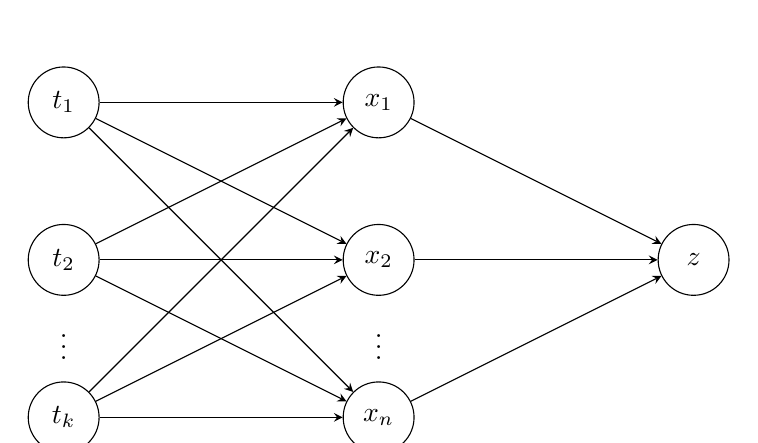
\begin{tikzpicture}[
    every node/.style={
        circle,
        draw,
        minimum size=0.9cm,
        inner sep=1pt
    },
    >=stealth
]

% input nodes
\node (t1) at (0,2) {$t_1$};
\node (t2) at (0,0) {$t_2$};
\node (tk) at (0,-2) {$t_k$};

% intermediate nodes
\node (x1) at (4,2) {$x_1$};
\node (x2) at (4,0) {$x_2$};
\node (xn) at (4,-2) {$x_n$};

% output
\node (z) at (8,0) {$z$};

% all-to-all input -> hidden
\foreach \a in {t1,t2,tk}
    \foreach \b in {x1,x2,xn}
        \draw[->] (\a) -- (\b);

% hidden -> output
\foreach \b in {x1,x2,xn}
    \draw[->] (\b) -- (z);

\node[draw=none] at (0,-1) {$\vdots$};
\node[draw=none] at (4,-1) {$\vdots$};

\end{tikzpicture}
\caption{여러 입력변수가 여러 중간 node를 거쳐 하나의 출력에 영향을 주는 구조}
\end{figure}

이제 특정 입력 $t_j$가 변할 때 출력 $z$가 얼마나 변하는지를
생각해 보자.

$t_j$에서 $z$까지 가는 경로는

\[
t_j\rightarrow x_1\rightarrow z,
\qquad
t_j\rightarrow x_2\rightarrow z,
\qquad
\ldots,
\qquad
t_j\rightarrow x_n\rightarrow z
\]

와 같이 여러 개가 있다.

따라서

\[
\boxed{
\frac{\partial z}{\partial t_j}
=
\frac{\partial z}{\partial x_1}
\frac{\partial x_1}{\partial t_j}
+
\frac{\partial z}{\partial x_2}
\frac{\partial x_2}{\partial t_j}
+\cdots+
\frac{\partial z}{\partial x_n}
\frac{\partial x_n}{\partial t_j}
}
\]

이다.

또는

\[
\boxed{
\frac{\partial z}{\partial t_j}
=
\sum_{i=1}^{n}
\frac{\partial z}{\partial x_i}
\frac{\partial x_i}{\partial t_j}
}
\]

로 쓸 수 있다.

% ------------------------------------------------------------
\subsection*{Gradient와 Jacobian을 이용한 표현}
% ------------------------------------------------------------

앞에서 다변수 chain rule을

\[
\boxed{
\frac{\partial z}{\partial t_j}
=
\sum_{i=1}^{n}
\frac{\partial z}{\partial x_i}
\frac{\partial x_i}{\partial t_j}
}
\qquad
(j=1,\ldots,k)
\]

로 나타내었다.

이제 이 관계를 vector와 matrix를 이용하여 보다 간결하게 표현해 보자.

다음과 같이
\[
\mathbf t
=
\begin{bmatrix}
t_1\\
t_2\\
\vdots\\
t_k
\end{bmatrix}
\in\mathbb R^k,
\qquad
\mathbf x
=
\begin{bmatrix}
x_1\\
x_2\\
\vdots\\
x_n
\end{bmatrix}
\in\mathbb R^n
\]
라고 하고,

\[
\mathbf x=\mathbf x(\mathbf t),
\qquad
z=z(\mathbf x)
\]

라고 하자.

즉,

\[
\mathbf t
\longrightarrow
\mathbf x
\longrightarrow
z
\]

와 같은 함수의 합성을 생각하고 있다.


\paragraph{Gradient.}

스칼라값 함수 $z=z(\mathbf x)$의 $\mathbf x$에 대한 gradient를
다음과 같이 column vector로 정의한다.

\[
\boxed{
\nabla_{\mathbf x}z
=
\begin{bmatrix}
\dfrac{\partial z}{\partial x_1}\\[0.6em]
\dfrac{\partial z}{\partial x_2}\\
\vdots\\
\dfrac{\partial z}{\partial x_n}
\end{bmatrix}
\in\mathbb R^n
}
\]

마찬가지로 $z$를 $\mathbf t$의 함수로 생각하면

\[
\boxed{
\nabla_{\mathbf t}z
=
\begin{bmatrix}
\dfrac{\partial z}{\partial t_1}\\[0.6em]
\dfrac{\partial z}{\partial t_2}\\
\vdots\\
\dfrac{\partial z}{\partial t_k}
\end{bmatrix}
\in\mathbb R^k
}
\]

이다.


\paragraph{Jacobian.}

벡터값 함수
\[
\mathbf x=\mathbf x(\mathbf t)
=
\begin{bmatrix}
x_1(\mathbf t)\\
x_2(\mathbf t)\\
\vdots\\
x_n(\mathbf t)
\end{bmatrix}
\]
의 Jacobian matrix를

\[
\boxed{
J_{\mathbf x}(\mathbf t)
=
\frac{\partial \mathbf x}{\partial \mathbf t}
=\frac{\partial (x_1,...x_n)}{\partial (t_1,...t_k)}=
\begin{bmatrix}
\dfrac{\partial x_1}{\partial t_1}
&
\dfrac{\partial x_1}{\partial t_2}
&
\cdots
&
\dfrac{\partial x_1}{\partial t_k}
\\[0.9em]
\dfrac{\partial x_2}{\partial t_1}
&
\dfrac{\partial x_2}{\partial t_2}
&
\cdots
&
\dfrac{\partial x_2}{\partial t_k}
\\
\vdots & \vdots & \ddots & \vdots
\\
\dfrac{\partial x_n}{\partial t_1}
&
\dfrac{\partial x_n}{\partial t_2}
&
\cdots
&
\dfrac{\partial x_n}{\partial t_k}
\end{bmatrix}
=
\begin{bmatrix}
(\nabla_{\mathbf t}x_1)^T\\
(\nabla_{\mathbf t}x_2)^T\\
\vdots\\
(\nabla_{\mathbf t}x_n)^T
\end{bmatrix}
\in\mathbb R^{n\times k}.
}
\]
로 정의한다.
따라서 그 transpose는

\[
\begin{aligned}
J_{\mathbf x}(\mathbf t)^T
&=
\begin{bmatrix}
\dfrac{\partial x_1}{\partial t_1}
&
\dfrac{\partial x_2}{\partial t_1}
&
\cdots
&
\dfrac{\partial x_n}{\partial t_1}
\\[0.9em]
\dfrac{\partial x_1}{\partial t_2}
&
\dfrac{\partial x_2}{\partial t_2}
&
\cdots
&
\dfrac{\partial x_n}{\partial t_2}
\\
\vdots & \vdots & \ddots & \vdots
\\
\dfrac{\partial x_1}{\partial t_k}
&
\dfrac{\partial x_2}{\partial t_k}
&
\cdots
&
\dfrac{\partial x_n}{\partial t_k}
\end{bmatrix}
\\[1em]
&=
\begin{bmatrix}
\nabla_{\mathbf t}x_1
&
\nabla_{\mathbf t}x_2
&
\cdots
&
\nabla_{\mathbf t}x_n
\end{bmatrix}.
\end{aligned}
\]
즉, 변수 $x_i$들의 벡터 $\mathbf{t}$에 대한 gradients를 열벡터로 갖는 행렬이다. 여기에 $\nabla_{\mathbf x}z$를 곱하면

\[
\begin{aligned}
J_{\mathbf x}(\mathbf t)^T\nabla_{\mathbf x}z
&=
\begin{bmatrix}
\displaystyle \sum_{i=1}^{n}\frac{\partial x_i}{\partial t_1}\frac{\partial z}{\partial x_i}\\[1em]
\displaystyle \sum_{i=1}^{n}\frac{\partial x_i}{\partial t_2}\frac{\partial z}{\partial x_i}\\
\vdots\\
\displaystyle \sum_{i=1}^{n}\frac{\partial x_i}{\partial t_k}\frac{\partial z}{\partial x_i}
\end{bmatrix}
=
\begin{bmatrix}
\dfrac{\partial z}{\partial t_1}\\[0.8em]
\dfrac{\partial z}{\partial t_2}\\
\vdots\\
\dfrac{\partial z}{\partial t_k}
\end{bmatrix}
=
\nabla_{\mathbf t}z = \frac{\partial z}{\partial \mathbf{t}}^T.
\end{aligned}
\]

위 식의 양변에 transpose를 취하면 Jacobian을 이용한 chain rule을 다음과 같이 compact하게 쓸 수 있다.

\[\frac{\partial z}{\partial \mathbf t} = \nabla_{\mathbf x}z ^T J_{\mathbf x}(\mathbf t) = \frac{\partial z}{\partial \mathbf x} \frac{\partial \mathbf x}{\partial \mathbf t}  \]

한편, gradient를 이용해서 표시하면,
\[ \nabla_{\mathbf t} z = \frac{\partial z}{\partial \mathbf t}^T =  J_{\mathbf x}(\mathbf t)^T\nabla_{\mathbf x}z = \frac{\partial \mathbf x}{\partial \mathbf t}^T \nabla_{\mathbf x}z \]


% ------------------------------------------------------------
\paragraph{작은 변화량에 대한 표현.}
% ------------------------------------------------------------

이제 작은 변화량
\[
\Delta\mathbf t
=
\begin{bmatrix}
\Delta t_1\\
\vdots\\
\Delta t_k
\end{bmatrix}
\]
을 생각하자.

스칼라함수 $z=z(\mathbf t)$의 일차근사에 의해

\[
\boxed{
\Delta z
\approx
(\nabla_{\mathbf t}z)^T
\Delta\mathbf t =  \frac{\partial z}{\partial \mathbf{t}} \Delta\mathbf t = \frac{\partial z}{\partial \mathb x}\frac{\partial \mathbf x}{\partial \mathbf t}\Delta \mathbf t
}
\]

이다. 즉 입력층의 작은 변화량 $\Delta\mathbf t$가 출력층의 작은 변화량 $\Delta z$로 전달되는 과정에서 Jacobian을 타고 근사된다.
반면 출력 $z$의 $\mathbf x$에 대한 gradient $\nabla_{\mathbf x}z$는 Jacobian의 transpose를 타고 입력층으로 $\nabla_{\mathbf t} z$로 전달된다.
\paragraph{Jacobian과 gradient의 방향}

스칼라값 함수 $z=z(\mathbf x)$에 대해서 Jacobian은
\[
\frac{\partial z}{\partial\mathbf x}
=
\begin{bmatrix}
\dfrac{\partial z}{\partial x_1}
&
\cdots
&
\dfrac{\partial z}{\partial x_n}
\end{bmatrix}
\]
와 같은 row vector이고, gradient는
\[
\nabla_{\mathbf x}z
=
\begin{bmatrix}
\dfrac{\partial z}{\partial x_1}\\
\vdots\\
\dfrac{\partial z}{\partial x_n}
\end{bmatrix}
\]
와 같은 column vector이다. 따라서
\[
\boxed{
\frac{\partial z}{\partial\mathbf x}
=
(\nabla_{\mathbf x}z)^T
}
\]
의 관계가 있다.

한편 벡터값 함수 $\mathbf x=\mathbf x(\mathbf t)$에 대해서는
\[
\Delta\mathbf x
\approx
\frac{\partial\mathbf x}{\partial\mathbf t}
\Delta\mathbf t
\]
이므로 작은 변화량은 Jacobian을 곱하면서 함수의 진행 방향으로 전달된다.

반대로 $z$가 scalar일 때 gradient는
\[
\boxed{
\nabla_{\mathbf t}z
=
\left(
\frac{\partial\mathbf x}{\partial\mathbf t}
\right)^T
\nabla_{\mathbf x}z
}
\]
이므로 뒤쪽 node에서 계산된 gradient는 Jacobian의 transpose를
곱하면서 앞쪽 node로 전달된다.

즉,
\[
\boxed{
\Delta\mathbf t
\;\xrightarrow{\;J\;}\;
\Delta\mathbf x,
\qquad
\nabla_{\mathbf x}z
\;\xrightarrow{\;J^T\;}\;
\nabla_{\mathbf t}z
}
\]

이다. 이러한 ``Jacobian은 forward 방향, Jacobian transpose는
gradient의 backward 방향''이라는 구조가 이후
backpropagation의 기본 원리가 된다.
%%%%%%%%%%%%%%%%%%%%%%%%%%%%%%%%%
\subsection*{예제}


\textbf{예 1.}

\[
z=z(x,y)=3x+5y+2,
\qquad
x=x(t,s)=2t+s+1,
\qquad
y=y(t,s)=3t-2s-1
\]

이라고 하자.

\paragraph{(1) 각 편도함수를 직접 계산하는 방법}

\[
z_t=z_xx_t+z_yy_t
=
3\cdot2+5\cdot3
=
21,
\]

\[
z_s=z_xx_s+z_yy_s
=
3\cdot1+5(-2)
=
-7.
\]

따라서

\[
\boxed{
\nabla_{(t,s)}z
=
\begin{bmatrix}
z_t\\
z_s
\end{bmatrix}
=
\begin{bmatrix}
21\\
-7
\end{bmatrix}
}
\]

이다.

한편 $x,y$를 $z$에 직접 대입하면

\[
z
=
3(2t+s+1)
+
5(3t-2s-1)
+
2
=
21t-7s
\]

이므로

\[
z_t=21,
\qquad
z_s=-7
\]

이고, 위의 결과와 일치한다.

\paragraph{(2) Jacobian과 gradient를 이용한 방법}

\[
\frac{\partial(x,y)}{\partial(t,s)}
=
\begin{bmatrix}
x_t & x_s\\
y_t & y_s
\end{bmatrix}
=
\begin{bmatrix}
2 & 1\\
3 & -2
\end{bmatrix},
\]

그리고

\[
\nabla_{(x,y)}z
=
\begin{bmatrix}
z_x\\
z_y
\end{bmatrix}
=
\begin{bmatrix}
3\\
5
\end{bmatrix}.
\]

따라서

\[
\boxed{
\nabla_{(t,s)}z
=
\left(
\frac{\partial(x,y)}{\partial(t,s)}
\right)^T
\nabla_{(x,y)}z
=
\begin{bmatrix}
2 & 3\\
1 & -2
\end{bmatrix}
\begin{bmatrix}
3\\
5
\end{bmatrix}
=
\begin{bmatrix}
21\\
-7
\end{bmatrix}
}
\]


\textbf{예 2.}

\[
z=z(x,y)=e^{2x}+\ln y,
\qquad
x=x(u,v)=u+2v,
\qquad
y=y(u,v)=u^2v
\]

에 대하여 $z$의 $u,v$에 대한 편도함수를 구해보자.

\begin{center}
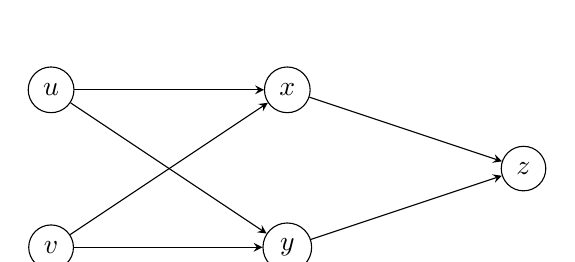
\begin{tikzpicture}[>=stealth]
\node[circle,draw] (u) at (0,1) {$u$};
\node[circle,draw] (v) at (0,-1) {$v$};

\node[circle,draw] (x) at (3,1) {$x$};
\node[circle,draw] (y) at (3,-1) {$y$};

\node[circle,draw] (z) at (6,0) {$z$};

\draw[->] (u) -- (x);
\draw[->] (u) -- (y);
\draw[->] (v) -- (x);
\draw[->] (v) -- (y);

\draw[->] (x) -- (z);
\draw[->] (y) -- (z);
\end{tikzpicture}
\end{center}

\paragraph{(1) 각 편도함수를 직접 계산하는 방법}

다변수 chain rule에 의해

\[
z_u=z_xx_u+z_yy_u,
\qquad
z_v=z_xx_v+z_yy_v.
\]

각 편도함수는

\[
z_x=2e^{2x},
\qquad
z_y=\frac{1}{y},
\qquad
x_u=1,
\qquad
x_v=2,
\qquad
y_u=2uv,
\qquad
y_v=u^2
\]

이므로

\[
z_u
=
z_xx_u+z_yy_u
=
2e^{2x}\cdot 1
+
\frac{1}{y}(2uv)
=
2e^{2u+4v}
+
\frac{2}{u},
\]

\[
z_v
=
z_xx_v+z_yy_v
=
2e^{2x}\cdot 2
+
\frac{1}{y}u^2
=
4e^{2u+4v}
+
\frac{1}{v}.
\]

따라서

\[
\boxed{
\nabla_{(u,v)}z
=
\begin{bmatrix}
z_u\\
z_v
\end{bmatrix}
=
\begin{bmatrix}
2e^{2u+4v}+\dfrac{2}{u}\\[0.8em]
4e^{2u+4v}+\dfrac{1}{v}
\end{bmatrix}
}
\]

이다.

\paragraph{(2) Jacobian과 gradient를 이용한 방법}

중간변수 $(x,y)$의 입력변수 $(u,v)$에 대한 Jacobian은

\[
\frac{\partial(x,y)}{\partial(u,v)}
=
\begin{bmatrix}
x_u & x_v\\
y_u & y_v
\end{bmatrix}
=
\begin{bmatrix}
1 & 2\\
2uv & u^2
\end{bmatrix}
\]

이고,

\[
\nabla_{(x,y)}z
=
\begin{bmatrix}
z_x\\
z_y
\end{bmatrix}
=
\begin{bmatrix}
2e^{2x}\\[0.4em]
\dfrac{1}{y}
\end{bmatrix}.
\]

따라서

\[
\begin{aligned}
\nabla_{(u,v)}z
&=
\left(
\frac{\partial(x,y)}{\partial(u,v)}
\right)^T
\nabla_{(x,y)}z
=
\begin{bmatrix}
1 & 2uv\\
2 & u^2
\end{bmatrix}
\begin{bmatrix}
2e^{2x}\\[0.4em]
\dfrac{1}{y}
\end{bmatrix}
\\[0.5em]
&=
\begin{bmatrix}
2e^{2x}+\dfrac{2uv}{y}\\[0.8em]
4e^{2x}+\dfrac{u^2}{y}
\end{bmatrix}
=
\begin{bmatrix}
2e^{2u+4v}+\dfrac{2}{u}\\[0.8em]
4e^{2u+4v}+\dfrac{1}{v}
\end{bmatrix}.
\end{aligned}
\]

즉, $z_u$와 $z_v$를 각각 계산하는 두 개의 chain rule을
Jacobian과 gradient의 하나의 matrix-vector multiplication으로
표현할 수 있다.

\paragraph{Gradient descent의 한 step}

이제 $z$를 $(u,v)$에 대한 목적함수로 생각하고,
gradient descent를 한 step 수행해보자.
초기값을
\[
u_0=-2,\qquad v_0=1
\]
로 두면
\[
x_0=u_0+2v_0=0,
\qquad
y_0=u_0^2v_0=4,
\]
따라서
\[
z_0=e^{2x_0}+\ln y_0
=1+\ln4
\approx2.3863.
\]

이제 $(u,v)$에 대한 $z$의 gradient를 직접 미분하여 구하지 않고,
computational graph
\[
(u,v)\longrightarrow(x,y)\longrightarrow z
\]
를 따라 뒤에서부터 차례로 계산해보자.

먼저 마지막 단계
\[
(x,y)\longrightarrow z
\]
에서의 gradient는
\[
\nabla_{(x,y)}z
=
\begin{bmatrix}
z_x\\
z_y
\end{bmatrix}
=
\begin{bmatrix}
2e^{2x}\\[0.4em]
\dfrac{1}{y}
\end{bmatrix}.
\]

$(x_0,y_0)=(0,4)$에서
\[
\nabla_{(x,y)}z
=
\begin{bmatrix}
2\\[0.3em]
\dfrac14
\end{bmatrix}.
\]

다음으로 앞 단계
\[
(u,v)\longrightarrow(x,y)
\]
의 Jacobian은
\[
\frac{\partial(x,y)}{\partial(u,v)}
=
\begin{bmatrix}
x_u & x_v\\
y_u & y_v
\end{bmatrix}
=
\begin{bmatrix}
1 & 2\\
2uv & u^2
\end{bmatrix}.
\]

$(u_0,v_0)=(-2,1)$에서
\[
\frac{\partial(x,y)}{\partial(u,v)}
=
\begin{bmatrix}
1 & 2\\
-4 & 4
\end{bmatrix}.
\]

따라서 chain rule의 matrix form을 이용하면
\[
\begin{aligned}
\nabla_{(u,v)}z
&=
\left(
\frac{\partial(x,y)}{\partial(u,v)}
\right)^T
\nabla_{(x,y)}z
\\
&=
\begin{bmatrix}
1 & -4\\
2 & 4
\end{bmatrix}
\begin{bmatrix}
2\\[0.3em]
\dfrac14
\end{bmatrix}
=
\begin{bmatrix}
1\\
5
\end{bmatrix}.
\end{aligned}
\]

즉,
\[
\boxed{
\nabla_{(x,y)}z
\quad\xrightarrow{\;
\left(\frac{\partial(x,y)}{\partial(u,v)}\right)^T
\;}
\quad
\nabla_{(u,v)}z
}
\]

와 같이 뒤쪽 node에서 구한 gradient가 Jacobian transpose와의
matrix-vector multiplication을 통하여 앞쪽 node로 전달된다.

이제 learning rate를 $\eta=0.01$로 두면
\[
\begin{aligned}
\begin{bmatrix}
u_1\\
v_1
\end{bmatrix}
&=
\begin{bmatrix}
u_0\\
v_0
\end{bmatrix}
-
\eta\nabla_{(u,v)}z
\\
&=
\begin{bmatrix}
-2\\
1
\end{bmatrix}
-
0.01
\begin{bmatrix}
1\\
5
\end{bmatrix}
=
\begin{bmatrix}
-2.01\\
0.95
\end{bmatrix}.
\end{aligned}
\]

새로운 값에서
\[
x_1=u_1+2v_1=-0.11,
\qquad
y_1=u_1^2v_1\approx3.8381,
\]
따라서
\[
z_1=e^{2x_1}+\ln y_1\approx2.1475.
\]

결과적으로
\[
\boxed{
z_0\approx2.3863
\quad\longrightarrow\quad
z_1\approx2.1475
}
\]
로 감소한다.

\bigskip

% ------------------------------------------------------------
\subsection{입력과 출력이 모두 여러 개인 경우}
% ------------------------------------------------------------

이제 출력도 하나가 아니라 여러 개라고 하자.

\[
\mathbf t
=
(t_1,\ldots,t_k),
\qquad
\mathbf x
=
(x_1,\ldots,x_n),
\qquad
\mathbf z
=
(z_1,\ldots,z_\ell)
\]

이고

\[
\mathbf t
\longrightarrow
\mathbf x
\longrightarrow
\mathbf z
\]

와 같은 계산구조를 생각하자.

각 출력 $z_r$는 모든 중간변수 $x_i$의 함수이고,
각 $x_i$는 다시 모든 입력변수 $t_j$의 함수이다.

그러면 각 pair $(z_r,t_j)$에 대하여

\[
\boxed{
\frac{\partial z_r}{\partial t_j}
=
\sum_{i=1}^{n}
\frac{\partial z_r}{\partial x_i}
\frac{\partial x_i}{\partial t_j}
}
\]

가 성립한다.

이 관계를 graph로 보면 다음과 같다.

\begin{figure}[ht]
\centering
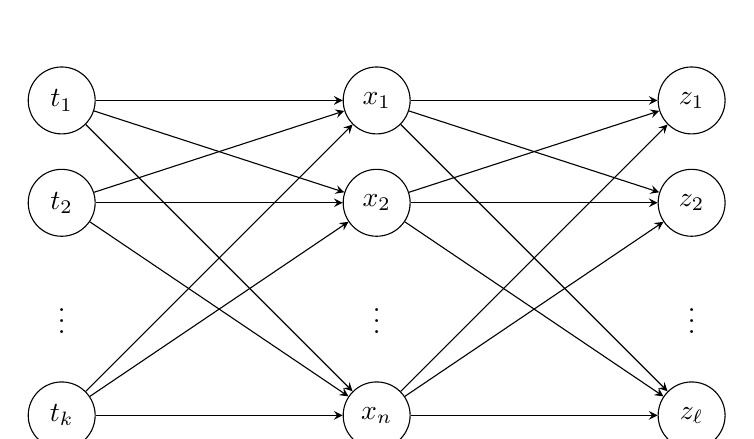
\begin{tikzpicture}[
    every node/.style={
        circle,
        draw,
        minimum size=0.85cm,
        inner sep=1pt
    },
    >=stealth
]

% input layer
\node (t1) at (0,2) {$t_1$};
\node (t2) at (0,0.7) {$t_2$};
\node (tk) at (0,-2) {$t_k$};

% middle layer
\node (x1) at (4,2) {$x_1$};
\node (x2) at (4,0.7) {$x_2$};
\node (xn) at (4,-2) {$x_n$};

% output layer
\node (z1) at (8,2) {$z_1$};
\node (z2) at (8,0.7) {$z_2$};
\node (zl) at (8,-2) {$z_\ell$};

\foreach \a in {t1,t2,tk}
    \foreach \b in {x1,x2,xn}
        \draw[->] (\a) -- (\b);

\foreach \a in {x1,x2,xn}
    \foreach \b in {z1,z2,zl}
        \draw[->] (\a) -- (\b);

\node[draw=none] at (0,-0.7) {$\vdots$};
\node[draw=none] at (4,-0.7) {$\vdots$};
\node[draw=none] at (8,-0.7) {$\vdots$};

\end{tikzpicture}
\caption{입력과 출력이 모두 여러 개인 vector-valued multivariable function}
\end{figure}

따라서 벡터값 함수에서도 본질은 동일하다.
각 출력 node $z_r$에 대해 하나씩 생각하면 된다.

예를 들어 $z_1$의 $t_2$에 대한 변화율을 알고 싶다면
$t_2$에서 $z_1$까지 연결되는 모든 경로를 찾고,

\[
t_2\rightarrow x_i\rightarrow z_1
\]

각 경로의 derivative들을 곱한 뒤, 모든 경로의 결과를 합하면 된다.


\paragraph{Jacobian을 이용한 합성함수 미분법}

이제 위의 관계를 Jacobian matrix를 이용하여 한꺼번에 표현해보자.
다음의 합성함수를 생각하자.

\[
\mathbf t=(t_1,\ldots,t_k)
\longrightarrow
\mathbf x=(x_1,\ldots,x_n)
\longrightarrow
\mathbf z=(z_1,\ldots,z_\ell).
\]

$\mathbf z$의 $\mathbf t$에 대한 Jacobian은

\[
\frac{\partial(z_1,\ldots,z_\ell)}
     {\partial(t_1,\ldots,t_k)}
=
\begin{bmatrix}
\dfrac{\partial z_1}{\partial t_1} &
\cdots &
\dfrac{\partial z_1}{\partial t_k}
\\[0.8em]
\vdots & \ddots & \vdots
\\[0.8em]
\dfrac{\partial z_\ell}{\partial t_1} &
\cdots &
\dfrac{\partial z_\ell}{\partial t_k}
\end{bmatrix}.
\]

한편 중간변수 $\mathbf x$를 기준으로 두 Jacobian을 각각 쓰면

\[
\frac{\partial(z_1,\ldots,z_\ell)}
     {\partial(x_1,\ldots,x_n)}
=
\begin{bmatrix}
\dfrac{\partial z_1}{\partial x_1} &
\cdots &
\dfrac{\partial z_1}{\partial x_n}
\\[0.8em]
\vdots & \ddots & \vdots
\\[0.8em]
\dfrac{\partial z_\ell}{\partial x_1} &
\cdots &
\dfrac{\partial z_\ell}{\partial x_n}
\end{bmatrix}
\]

이고,

\[
\frac{\partial(x_1,\ldots,x_n)}
     {\partial(t_1,\ldots,t_k)}
=
\begin{bmatrix}
\dfrac{\partial x_1}{\partial t_1} &
\cdots &
\dfrac{\partial x_1}{\partial t_k}
\\[0.8em]
\vdots & \ddots & \vdots
\\[0.8em]
\dfrac{\partial x_n}{\partial t_1} &
\cdots &
\dfrac{\partial x_n}{\partial t_k}
\end{bmatrix}.
\]

이 두 Jacobian을 곱한 행렬의 $(r,j)$번째 원소는

\[
\sum_{i=1}^{n}
\frac{\partial z_r}{\partial x_i}
\frac{\partial x_i}{\partial t_j}
=
\frac{\partial z_r}{\partial t_j}.
\]

따라서

\[
\boxed{
\frac{\partial(z_1,\ldots,z_\ell)}
     {\partial(t_1,\ldots,t_k)}
=
\frac{\partial(z_1,\ldots,z_\ell)}
     {\partial(x_1,\ldots,x_n)}
\frac{\partial(x_1,\ldots,x_n)}
     {\partial(t_1,\ldots,t_k)}
}
\]

를 얻는다.

즉, 차원으로 보면

\[
(\ell\times k)
=
(\ell\times n)(n\times k)
\]

이고, 다변수함수의 chain rule은 Jacobian matrix의 곱으로
compact하게 표현된다.

또한 작은 변화량을 생각하면

\[
\Delta\mathbf x
\approx
\frac{\partial\mathbf x}{\partial\mathbf t}
\Delta\mathbf t,
\qquad
\Delta\mathbf z
\approx
\frac{\partial\mathbf z}{\partial\mathbf x}
\Delta\mathbf x,
\]

이므로

\[
\boxed{
\Delta\mathbf z
\approx
\frac{\partial\mathbf z}{\partial\mathbf x}
\frac{\partial\mathbf x}{\partial\mathbf t}
\Delta\mathbf t
=
\frac{\partial\mathbf z}{\partial\mathbf t}
\Delta\mathbf t
}
\]

가 된다.



% ------------------------------------------------------------
\subsection{여러 층으로 이루어진 함수의 합성}
% ------------------------------------------------------------

이제 중간 node가 한 층이 아니라 여러 층 존재한다고 하자.

예를 들어

\[
\mathbf t
\longrightarrow
\mathbf x
\longrightarrow
\mathbf y
\longrightarrow
\mathbf z
\]

와 같은 계산구조를 생각할 수 있다.

\begin{figure}[ht]
\centering
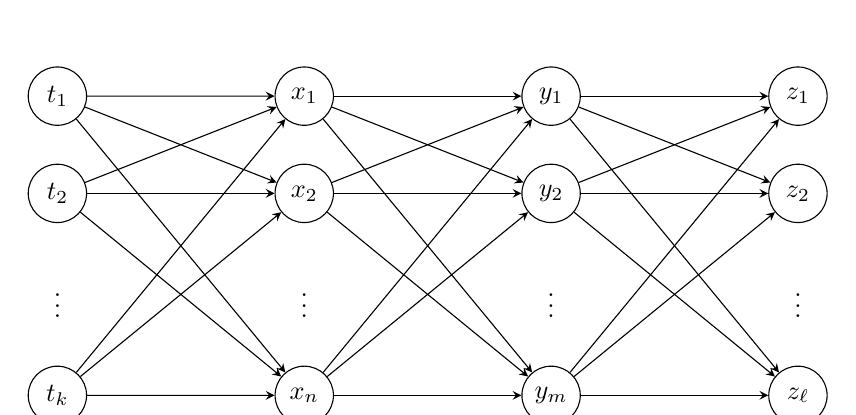
\begin{tikzpicture}[
    every node/.style={
        circle,
        draw,
        minimum size=0.78cm,
        inner sep=1pt
    },
    >=stealth,
    scale=0.95,
    transform shape
]

% t layer
\node (t1) at (0,2) {$t_1$};
\node (t2) at (0,0.7) {$t_2$};
\node (tk) at (0,-2) {$t_k$};

% x layer
\node (x1) at (3.3,2) {$x_1$};
\node (x2) at (3.3,0.7) {$x_2$};
\node (xn) at (3.3,-2) {$x_n$};

% y layer
\node (y1) at (6.6,2) {$y_1$};
\node (y2) at (6.6,0.7) {$y_2$};
\node (ym) at (6.6,-2) {$y_m$};

% z layer
\node (z1) at (9.9,2) {$z_1$};
\node (z2) at (9.9,0.7) {$z_2$};
\node (zl) at (9.9,-2) {$z_\ell$};

\foreach \a in {t1,t2,tk}
    \foreach \b in {x1,x2,xn}
        \draw[->] (\a) -- (\b);

\foreach \a in {x1,x2,xn}
    \foreach \b in {y1,y2,ym}
        \draw[->] (\a) -- (\b);

\foreach \a in {y1,y2,ym}
    \foreach \b in {z1,z2,zl}
        \draw[->] (\a) -- (\b);

\node[draw=none] at (0,-0.7) {$\vdots$};
\node[draw=none] at (3.3,-0.7) {$\vdots$};
\node[draw=none] at (6.6,-0.7) {$\vdots$};
\node[draw=none] at (9.9,-0.7) {$\vdots$};

\end{tikzpicture}
\caption{여러 층의 node로 이루어진 함수의 반복적인 합성}
\end{figure}

예를 들어 $z_r$의 $t_j$에 대한 미분을 생각하면,
$t_j$에서 $z_r$까지 가는 경로는 매우 많아진다.

하나의 경로

\[
t_j
\longrightarrow
x_i
\longrightarrow
y_q
\longrightarrow
z_r
\]

를 따라 전달되는 변화율은

\[
\frac{\partial z_r}{\partial y_q}
\frac{\partial y_q}{\partial x_i}
\frac{\partial x_i}{\partial t_j}
\]

이고, 가능한 모든 $i,q$를 통하는 경로를 합하면

\[
\boxed{
\frac{\partial z_r}{\partial t_j}
=
\sum_{q}
\sum_{i}
\frac{\partial z_r}{\partial y_q}
\frac{\partial y_q}{\partial x_i}
\frac{\partial x_i}{\partial t_j}
}
\]

를 얻는다.

따라서 층의 수가 증가하더라도 기본 원리는 변하지 않는다.

\subsection*{예}

다음과 같은 합성함수를 생각하자.

\[
(t_1,t_2)
\longrightarrow
(x_1,x_2)
\longrightarrow
(y_1,y_2)
\longrightarrow
z,
\]

여기서

\[
x_1=t_1+t_2,\qquad
x_2=t_1-t_2,
\]

\[
y_1=x_1^2+x_2,\qquad
y_2=x_1+2x_2,
\]

\[
z=y_1^2+y_2
\]

라고 하자.

\begin{center}
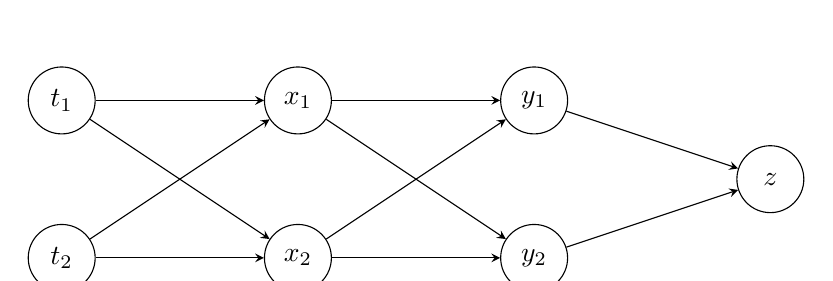
\begin{tikzpicture}[>=stealth,
    every node/.style={
        circle,
        draw,
        minimum size=0.85cm,
        inner sep=1pt
    }]

% input
\node (t1) at (0,1) {$t_1$};
\node (t2) at (0,-1) {$t_2$};

% first layer
\node (x1) at (3,1) {$x_1$};
\node (x2) at (3,-1) {$x_2$};

% second layer
\node (y1) at (6,1) {$y_1$};
\node (y2) at (6,-1) {$y_2$};

% output
\node (z) at (9,0) {$z$};

\foreach \a in {t1,t2}
    \foreach \b in {x1,x2}
        \draw[->] (\a) -- (\b);

\foreach \a in {x1,x2}
    \foreach \b in {y1,y2}
        \draw[->] (\a) -- (\b);

\foreach \a in {y1,y2}
    \draw[->] (\a) -- (z);

\end{tikzpicture}
\end{center}

각 층의 Jacobian은

\[
\frac{\partial(x_1,x_2)}
     {\partial(t_1,t_2)}
=
\begin{bmatrix}
1&1\\
1&-1
\end{bmatrix},
\]

\[
\frac{\partial(y_1,y_2)}
     {\partial(x_1,x_2)}
=
\begin{bmatrix}
2x_1&1\\
1&2
\end{bmatrix},
\]

그리고 마지막 출력 $z$의 $(y_1,y_2)$에 대한 Jacobian은

\[
\frac{\partial z}{\partial(y_1,y_2)}
=
\begin{bmatrix}
2y_1&1
\end{bmatrix}.
\]

따라서 Jacobian의 chain rule에 의해

\[
\boxed{
\frac{\partial z}{\partial(t_1,t_2)}
=
\frac{\partial z}{\partial(y_1,y_2)}
\frac{\partial(y_1,y_2)}{\partial(x_1,x_2)}
\frac{\partial(x_1,x_2)}{\partial(t_1,t_2)}
}
\]

이다.

차원을 확인하면

\[
(1\times2)(2\times2)(2\times2)
=
(1\times2)
\]

로 정확히 맞는다.


한편 gradient는 scalar 함수의 Jacobian을 transpose한 것이므로,

\[
\nabla_{(t_1,t_2)}z
=
\left(
\frac{\partial z}{\partial(t_1,t_2)}
\right)^T.
\]

앞의 Jacobian chain rule을 transpose하면

\[
\begin{aligned}
\nabla_{(t_1,t_2)}z
&=
\left[
\frac{\partial z}{\partial(y_1,y_2)}
\frac{\partial(y_1,y_2)}{\partial(x_1,x_2)}
\frac{\partial(x_1,x_2)}{\partial(t_1,t_2)}
\right]^T
\\[0.5em]
&=
\left(
\frac{\partial(x_1,x_2)}{\partial(t_1,t_2)}
\right)^T
\left(
\frac{\partial(y_1,y_2)}{\partial(x_1,x_2)}
\right)^T
\left(
\frac{\partial z}{\partial(y_1,y_2)}
\right)^T
\\[0.5em]
&=
\left(
\frac{\partial(x_1,x_2)}{\partial(t_1,t_2)}
\right)^T
\left(
\frac{\partial(y_1,y_2)}{\partial(x_1,x_2)}
\right)^T
\nabla_{(y_1,y_2)}z.
\end{aligned}
\]

즉 gradient는 출력에서 시작하여

\[
\boxed{
\nabla_{(y_1,y_2)}z
\;\xrightarrow{\;
\left(\frac{\partial(y_1,y_2)}{\partial(x_1,x_2)}\right)^T
\;}
\nabla_{(x_1,x_2)}z
\;\xrightarrow{\;
\left(\frac{\partial(x_1,x_2)}{\partial(t_1,t_2)}\right)^T
\;}
\nabla_{(t_1,t_2)}z
}
\]

와 같이 각 층의 Jacobian transpose를 곱하면서 graph의 반대 방향으로 전달된다.

% =================================================
\section{Linear Regression을 Computational Graph로 다시 보기}
% =================================================

이제 이미 알고 있는 선형회귀를 chain rule의 관점에서 다시 해석한다.
데이터
\[
(x_i,y_i),\qquad i=1,\ldots,N
\]
가 주어졌다고 하자.

모델은
\[
\widehat y_i=wx_i+b
\]
이고, mean squared error는
\[
\boxed{
L(w,b)
=
\frac{1}{N}
\sum_{i=1}^N
(\widehat y_i-y_i)^2
}
\]
이다.

\subsection{한 개의 데이터에 대한 계산 그래프}

먼저 하나의 datum $(x,y)$만 생각하자.
\[
\widehat y=wx+b,
\qquad
e=\widehat y-y,
\qquad
\ell=e^2.
\]

\begin{center}
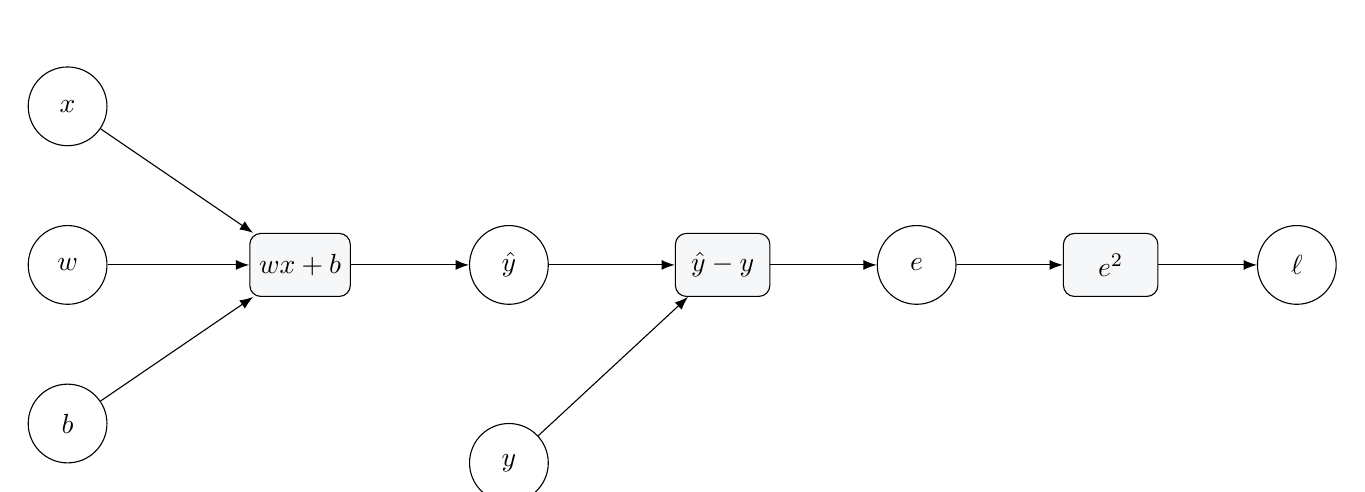
\begin{tikzpicture}[
>=Latex,
node distance=1.55cm and 1.6cm,
var/.style={draw,circle,minimum size=10mm,inner sep=1pt},
op/.style={draw,rounded corners,minimum height=8mm,minimum width=12mm,fill=softgray}
]
\node[var] (x) {$x$};
\node[var,below=10mm of x] (w) {$w$};
\node[var,below=10mm of w] (b) {$b$};
\node[op,right=1.8cm of w] (aff) {$wx+b$};
\node[var,right=1.5cm of aff] (yh) {$\hat y$};
\node[var,below=15mm of yh] (yt) {$y$};
\node[op,right=1.6cm of yh] (sub) {$\hat y-y$};
\node[var,right=1.35cm of sub] (e) {$e$};
\node[op,right=1.35cm of e] (sq) {$e^2$};
\node[var,right=1.25cm of sq] (ell) {$\ell$};
\draw[->] (x)--(aff);
\draw[->] (w)--(aff);
\draw[->] (b)--(aff);
\draw[->] (aff)--(yh);
\draw[->] (yh)--(sub);
\draw[->] (yt)--(sub);
\draw[->] (sub)--(e);
\draw[->] (e)--(sq);
\draw[->] (sq)--(ell);
\end{tikzpicture}
\end{center}

Forward 계산은 단순히
\[
(w,b,x)
\longrightarrow
\widehat y
\longrightarrow
e
\longrightarrow
\ell
\]
순서로 진행한다.

\subsection{Local derivatives}

각 edge에 해당하는 local derivative를 계산하면
\[
\frac{\partial \ell}{\partial e}=2e,
\qquad
\frac{\partial e}{\partial \widehat y}=1,
\]
그리고
\[
\frac{\partial \widehat y}{\partial w}=x,
\qquad
\frac{\partial \widehat y}{\partial b}=1.
\]

따라서 chain rule에 의해
\[
\boxed{
\frac{\partial \ell}{\partial w}
=
\frac{\partial \ell}{\partial e}
\frac{\partial e}{\partial \widehat y}
\frac{\partial \widehat y}{\partial w}
=
2ex
}
\]
이고
\[
\boxed{
\frac{\partial \ell}{\partial b}
=
\frac{\partial \ell}{\partial e}
\frac{\partial e}{\partial \widehat y}
\frac{\partial \widehat y}{\partial b}
=
2e
}
\]
이다.

즉, loss에서 시작하여 computational graph를 반대 방향으로 따라가면서
각 edge의 local derivative를 곱한다.

\subsection{전체 데이터에 대한 gradient}

\[
L(w,b)=\frac1N\sum_{i=1}^N\ell_i
\]
이므로
\[
\frac{\partial L}{\partial w}
=
\frac1N\sum_{i=1}^N
\frac{\partial \ell_i}{\partial w}
=
\boxed{
\frac{2}{N}\sum_{i=1}^N(\widehat y_i-y_i)x_i
}
\]
이고
\[
\frac{\partial L}{\partial b}
=
\boxed{
\frac{2}{N}\sum_{i=1}^N(\widehat y_i-y_i)
}
\]
이다.

Gradient vector는
\[
\grad L(w,b)
=
\begin{bmatrix}
\partial L/\partial w\\[0.2em]
\partial L/\partial b
\end{bmatrix}.
\]

Gradient descent는
\[
\boxed{
\begin{bmatrix}
w_{k+1}\\ b_{k+1}
\end{bmatrix}
=
\begin{bmatrix}
w_k\\ b_k
\end{bmatrix}
-
\eta
\begin{bmatrix}
\partial L/\partial w\\
\partial L/\partial b
\end{bmatrix}
}
\]
이다.

\begin{keybox}[여기에서 구분해야 할 두 가지]
\textbf{Backpropagation}은 gradient를 \emph{계산하는 방법}이다.

\textbf{Gradient descent}는 계산된 gradient를 사용하여 parameter를 \emph{업데이트하는 방법}이다.

즉,
\[
\boxed{
\text{Forward}
\rightarrow
\text{Loss}
\rightarrow
\text{Backward}
\rightarrow
\text{Gradient}
\rightarrow
\text{Parameter Update}
}
\]
이다.
\end{keybox}


% =================================================
\section{숫자로 Gradient의 흐름을 끝까지 추적해 보기}
% =================================================

다음 세 개의 데이터를 생각하자.
\[
(1,1),\qquad(2,2),\qquad(3,2).
\]
초기값을
\[
w_0=1,\qquad b_0=1
\]
로 둔다. 그러면 $\widehat y=x+1$이다.

\begin{center}
\begin{tabular}{c|c|c|c|c|c|c}
\toprule
$x_i$ & $y_i$ & $\widehat y_i$ & $e_i$ & $\ell_i=e_i^2$ & $\partial\ell_i/\partial w$ & $\partial\ell_i/\partial b$\\
\midrule
1 & 1 & 2 & 1 & 1 & $2(1)(1)=2$ & $2(1)=2$\\
2 & 2 & 3 & 1 & 1 & $2(1)(2)=4$ & $2(1)=2$\\
3 & 2 & 4 & 2 & 4 & $2(2)(3)=12$ & $2(2)=4$\\
\bottomrule
\end{tabular}
\end{center}

따라서
\[
\frac{\partial L}{\partial w}
=
\frac{2+4+12}{3}=6,
\qquad
\frac{\partial L}{\partial b}
=
\frac{2+2+4}{3}=\frac{8}{3}.
\]

학습률을 $\eta=0.03$이라 하면 한 번의 gradient descent step은
\[
w_1=1-0.03(6)=0.82,
\]
\[
b_1=1-0.03\left(\frac83\right)=0.92.
\]

% =================================================
\section{3차시 실습: NumPy Hard Coding}
% =================================================

이번 실습에서는 PyTorch의 autograd를 사용하지 않는다.
수학적으로 유도한 모든 값을 직접 계산한다.

\subsection{실습 목표}

코드 안에서 다음 다섯 단계를 눈으로 확인한다.
\[
\boxed{
\text{data}
\rightarrow
\text{forward}
\rightarrow
\text{loss}
\rightarrow
\text{backward}
\rightarrow
\text{parameter update}
}
\]

\subsection{Step 1. 데이터와 모델}

\begin{lstlisting}
import numpy as np
import matplotlib.pyplot as plt

x = np.array([1., 2., 3., 4., 5.])
y = np.array([2.2, 2.8, 3.6, 4.5, 5.1])

w = 0.0
b = 0.0
learning_rate = 0.01
epochs = 200
N = len(x)
\end{lstlisting}

모델은
\[
\widehat y=wx+b
\]
이다.

\subsection{Step 2. Forward propagation}

\begin{lstlisting}
y_hat = w * x + b
error = y_hat - y
loss = np.mean(error**2)
\end{lstlisting}

이 세 줄은 수학적으로
\[
\widehat y_i=wx_i+b,
\qquad
e_i=\widehat y_i-y_i,
\qquad
L=\frac1N\sum_i e_i^2
\]
를 계산한다.

\subsection{Step 3. Backward propagation}

이번에는 최종 공식을 바로 쓰지 말고 local derivative를 코드에 그대로 남긴다.

\begin{lstlisting}
dl_de = 2.0 * error

de_dyhat = 1.0

dyhat_dw = x
dyhat_db = 1.0

# Chain rule for each sample
sample_grad_w = dl_de * de_dyhat * dyhat_dw
sample_grad_b = dl_de * de_dyhat * dyhat_db

# Mean over all samples
dL_dw = np.mean(sample_grad_w)
dL_db = np.mean(sample_grad_b)
\end{lstlisting}

수학식과 정확히 대응시키면
\[
\frac{\partial \ell_i}{\partial w}
=
\underbrace{\frac{\partial \ell_i}{\partial e_i}}_{2e_i}
\underbrace{\frac{\partial e_i}{\partial \widehat y_i}}_{1}
\underbrace{\frac{\partial \widehat y_i}{\partial w}}_{x_i}
\]
이고,
\[
\frac{\partial \ell_i}{\partial b}
=
\underbrace{\frac{\partial \ell_i}{\partial e_i}}_{2e_i}
\underbrace{\frac{\partial e_i}{\partial \widehat y_i}}_{1}
\underbrace{\frac{\partial \widehat y_i}{\partial b}}_{1}.
\]

\subsection{Step 4. Parameter update}

\begin{lstlisting}
w -= learning_rate * dL_dw
b -= learning_rate * dL_db
\end{lstlisting}

즉,
\[
w\leftarrow w-\eta\frac{\partial L}{\partial w},
\qquad
b\leftarrow b-\eta\frac{\partial L}{\partial b}.
\]

\subsection{Step 5. 전체 training loop}

\begin{lstlisting}
import numpy as np
import matplotlib.pyplot as plt

x = np.array([1., 2., 3., 4., 5.])
y = np.array([2.2, 2.8, 3.6, 4.5, 5.1])

w = 0.0
b = 0.0
learning_rate = 0.01
epochs = 200
N = len(x)

loss_history = []

for epoch in range(epochs):
    # ---------------------------------
    # 1. Forward
    # ---------------------------------
    y_hat = w * x + b
    error = y_hat - y
    loss = np.mean(error**2)

    # ---------------------------------
    # 2. Backward: local derivatives
    # ---------------------------------
    dl_de = 2.0 * error
    de_dyhat = 1.0
    dyhat_dw = x
    dyhat_db = 1.0

    sample_grad_w = dl_de * de_dyhat * dyhat_dw
    sample_grad_b = dl_de * de_dyhat * dyhat_db

    dL_dw = np.mean(sample_grad_w)
    dL_db = np.mean(sample_grad_b)

    # ---------------------------------
    # 3. Gradient-descent step
    # ---------------------------------
    w -= learning_rate * dL_dw
    b -= learning_rate * dL_db

    loss_history.append(loss)

    if epoch % 20 == 0:
        print(
            f"epoch={epoch:3d}, loss={loss:.6f}, "
            f"w={w:.4f}, b={b:.4f}, "
            f"dL_dw={dL_dw:.4f}, dL_db={dL_db:.4f}"
        )

print("final w =", w)
print("final b =", b)

# Plot fitted line
x_plot = np.linspace(0.5, 5.5, 100)
y_plot = w * x_plot + b

plt.figure(figsize=(10, 4))

plt.subplot(1, 2, 1)
plt.scatter(x, y, label="data")
plt.plot(x_plot, y_plot, label="fitted line")
plt.xlabel("x")
plt.ylabel("y")
plt.legend()
plt.grid(True)

plt.subplot(1, 2, 2)
plt.plot(loss_history)
plt.xlabel("epoch")
plt.ylabel("MSE loss")
plt.grid(True)

plt.tight_layout()
plt.show()
\end{lstlisting}

\subsection{Step 6. Gradient check: 우리가 유도한 미분이 맞는가?}

Backpropagation으로 계산한 gradient를 numerical differentiation과 비교해 볼 수 있다.

\begin{lstlisting}
def compute_loss(x, y, w, b):
    y_hat = w * x + b
    return np.mean((y_hat - y)**2)


def numerical_gradient(x, y, w, b, h=1e-5):
    dL_dw = (
        compute_loss(x, y, w + h, b)
        - compute_loss(x, y, w - h, b)
    ) / (2*h)

    dL_db = (
        compute_loss(x, y, w, b + h)
        - compute_loss(x, y, w, b - h)
    ) / (2*h)

    return dL_dw, dL_db
\end{lstlisting}

예를 들어 같은 $(w,b)$에서
\[
\left(\frac{\partial L}{\partial w},\frac{\partial L}{\partial b}\right)_{\text{backprop}}
\approx
\left(\frac{\partial L}{\partial w},\frac{\partial L}{\partial b}\right)_{\text{finite difference}}
\]
인지 확인한다.


% =================================================
\section{연습문제}
% =================================================

\begin{enumerate}[label=\textbf{\arabic*.},leftmargin=2.2em]
\item 다음 함수의 도함수를 중간 변수를 명시하여 chain rule로 계산하라.
\[
y=\log\left(1+e^{2x}\right).
\]

\item
\[
z=x^2y+\sin y,
\qquad
x=t^2,
\qquad
y=e^t
\]
일 때 $dz/dt$를 구하라.

\item 다음 vector-valued function의 Jacobian을 구하라.
\[
F(x_1,x_2)
=
\begin{bmatrix}
x_1^2+x_2\\
\sin(x_1x_2)
\end{bmatrix}.
\]

\item 선형회귀에서 loss를
\[
L(w,b)=\frac{1}{2N}\sum_{i=1}^N(wx_i+b-y_i)^2
\]
로 정의하면 $\partial L/\partial w$, $\partial L/\partial b$는 어떻게 바뀌는가?
$1/2$를 붙이는 이유를 설명하라.

\item 데이터
\[
(1,2),\qquad(2,2),\qquad(4,5)
\]
와 초기값 $w=1/2$, $b=1$이 주어졌다고 하자. 한 번의 forward/backward를 직접 계산하여
$\partial L/\partial w$, $\partial L/\partial b$를 구하고, $\eta=0.05$로 한 번 update한 $(w,b)$를 계산하라.

\item 코드에서 $\texttt{learning\_rate}$를 $0.001$, $0.01$, $0.1$, $0.5$로 바꾸어 loss history를 비교하라.
학습률이 너무 작거나 너무 클 때 어떤 현상이 나타나는지 설명하라.
\end{enumerate}


\section*{참고문헌}
\begin{itemize}
\item M. P. Deisenroth, A. A. Faisal, C. S. Ong, \emph{Mathematics for Machine Learning}, Cambridge University Press, Chapter 5 (Vector Calculus), especially Sections 5.2, 5.3, and 5.6.
\end{itemize}

\end{document}
